% !Mode:: "TeX:UTF-8"
\def\usewhat{pdflatex}                               % 定义编译方式 dvipdfmx 或者 pdflatex,默认为 dvipdfmx
                                                     % 方式编译,如果需要修改,只需改变花括号中的内容即可。
\documentclass[12pt,openany,a4paper,twoside]{book} %原本的设置
%\documentclass[12pt,openany,twoside]{book}           % 本科生毕业论文通常采用单页排版
% !Mode:: "TeX:UTF-8"
%  Authors: 张井   Jing Zhang: prayever@gmail.com     天津大学2010级管理与经济学部信息管理与信息系统专业硕士生
%           余蓝涛 Lantao Yu: lantaoyu1991@gmail.com  天津大学2008级精密仪器与光电子工程学院测控技术与仪器专业本科生

%%%%%%%%%% Package %%%%%%%%%%%%
\usepackage{graphicx}                       % 支持插图处理
\usepackage[a4paper,text={146.4true mm,239.2 true mm},top= 26.2true mm,left=31.8 true mm,head=6true mm,headsep=6.5true mm,foot=16.5true mm]{geometry}
                                            % 支持版面尺寸设置
\usepackage[squaren]{SIunits}               % 支持国际标准单位

\usepackage{titlesec}                       % 控制标题的宏包
\usepackage{titletoc}                       % 控制目录的宏包
\usepackage{fancyhdr}                       % fancyhdr宏包 支持页眉和页脚的相关定义
\usepackage[UTF8]{ctex}                     % 支持中文显示
\usepackage{CJKpunct}                       % 精细调整中文的标点符号
\usepackage{color}                          % 支持彩色
\usepackage{amsmath}                        % AMSLaTeX宏包 用来排出更加漂亮的公式
\usepackage{amssymb}                        % 数学符号生成命令
\usepackage[below]{placeins}    %允许上一个section的浮动图形出现在下一个section的开始部分,还提供\FloatBarrier命令,使所有未处理的浮动图形立即被处理
\usepackage{multirow}                       % 使用Multirow宏包,使得表格可以合并多个row格
\usepackage{booktabs}                       % 表格,横的粗线;\specialrule{1pt}{0pt}{0pt}
\usepackage{longtable}                      % 支持跨页的表格。
\usepackage{tabularx}                       % 自动设置表格的列宽
\usepackage{subfigure}                      % 支持子图 %centerlast 设置最后一行是否居中
\usepackage[subfigure]{ccaption}            % 支持子图的中文标题
\usepackage[sort&compress,numbers]{natbib}  % 支持引用缩写的宏包
\usepackage{enumitem}                       % 使用enumitem宏包,改变列表项的格式
\usepackage{calc}                           % 长度可以用+ - * / 进行计算
\usepackage{txfonts}                        % 字体宏包
\usepackage{bm}                             % 处理数学公式中的黑斜体的宏包
\usepackage[amsmath,thmmarks,hyperref]{ntheorem}  % 定理类环境宏包,其中 amsmath 选项用来兼容 AMS LaTeX 的宏包
\usepackage{CJKnumb}                        % 提供将阿拉伯数字转换成中文数字的命令
\usepackage{indentfirst}                    % 首行缩进宏包
\usepackage{CJKutf8}                        % 用在UTF8编码环境下,它可以自动调用CJK,同时针对UTF8编码作了设置
%\usepackage{hypbmsec}                      % 用来控制书签中标题显示内容
%\usepackage{enumerate}                      % 用于控制排序列表的编号样式
\newcommand{\tabincell}[2]{\begin{tabular}{@{}#1@{}}#2\end{tabular}}
\usepackage{xcolor}
%支持代码环境
\usepackage{listings}
\lstset{numbers=left,
language=[ANSI]{C},
numberstyle=\tiny,
extendedchars=false,
showstringspaces=false,
breakatwhitespace=false,
breaklines=true,
captionpos=b,
keywordstyle=\color{blue!70},
commentstyle=\color{red!50!green!50!blue!50},
frame=shadowbox,
rulesepcolor=\color{red!20!green!20!blue!20}
}
%支持算法环境
\usepackage[longend,linesnumbered,boxed,ruled,lined]{algorithm2e}
%\usepackage{algorithmic}

\usepackage{array}
\newcommand{\PreserveBackslash}[1]{\let\temp=\\#1\let\\=\temp}
\newcolumntype{C}[1]{>{\PreserveBackslash\centering}p{#1}}
\newcolumntype{R}[1]{>{\PreserveBackslash\raggedleft}p{#1}}
\newcolumntype{L}[1]{>{\PreserveBackslash\raggedright}p{#1}}

% 生成有书签的 pdf 及其生成方式。通常可以在 tjumain.tex 文件的第一行选择 pdflatex 或者是 dvipdfmx 编译手段。如果选择前者,则使用 pdflatex + pdflatex 编译; 如果选择后者,在编译的时候选择 latex + bibtex + latex + latex 编译。出现混淆的时候,系统会报错。
% 如果您的pdf制作中文书签有乱码使用如下命令,就可以解决了
\def\atemp{dvipdfmx}\ifx\atemp\usewhat
\usepackage[dvipdfmx,unicode,               % dvipdfmx 编译, 加入了中文复制,粘贴支持引擎。
            pdfstartview=FitH,
            bookmarksnumbered=true,
            bookmarksopen=true,
            colorlinks=false,
            pdfborder={0 0 1},
            citecolor=blue,
            linkcolor=black,
            anchorcolor=green,
            urlcolor=blue,
            breaklinks=true
            ]{hyperref}
\fi

\def\atemp{pdflatex}\ifx\atemp\usewhat
\usepackage{cmap}                           % pdflatex 编译时,可以生成可复制、粘贴的中文 PDF 文档, 缺点是在Windows上显示时效果不大好,字体发虚
\usepackage[pdftex,unicode,
            %CJKbookmarks=true,
            bookmarksnumbered=true,
            bookmarksopen=true,
            colorlinks=false,
            pdfborder={0 0 0},%pdfborder={0 0 1}就能显示红色框
            citecolor=blue,
            linkcolor=red,
            anchorcolor=green,
            urlcolor=blue,
            breaklinks=true
            ]{hyperref}
\fi

\usepackage{setspace}   % 用于目录设置行距


\usepackage{caption}

                                % 定义本文所使用宏包
\usepackage{graphicx}
\usepackage{subfigure}
\usepackage{epstopdf}                                 %支持eps图片转换成PDF格式
\usepackage{tipa}
\graphicspath{{figures/}}                            % 定义所有的 .eps 文件在 figures 子目录下
\begin{document}                                     % 开始全文
\begin{CJK*}{UTF8}{song}                             % 开始中文字体使用
% !Mode:: "TeX:UTF-8"

%%%%%%%%%%%%%%%%% Fonts Definition and Basics %%%%%%%%%%%%%%%%%
\newcommand{\song}{\CJKfamily{song}}    % 宋体
\newcommand{\fs}{\CJKfamily{fs}}        % 仿宋体
\newcommand{\kai}{\CJKfamily{kai}}      % 楷体
\newcommand{\hei}{\CJKfamily{hei}}      % 黑体
\newcommand{\li}{\CJKfamily{li}}        % 隶书
\newcommand{\chuhao}{\fontsize{28pt}{28pt}\selectfont}       % 初号, 单倍行距
\newcommand{\yihao}{\fontsize{26pt}{26pt}\selectfont}       % 一号, 单倍行距
\newcommand{\xiaoyi}{\fontsize{24pt}{24pt}\selectfont}      % 小一, 单倍行距
\newcommand{\erhao}{\fontsize{22pt}{1.25\baselineskip}\selectfont}       % 二号, 1.25倍行距
\newcommand{\xiaoer}{\fontsize{18pt}{18pt}\selectfont}      % 小二, 单倍行距
\newcommand{\sanhao}{\fontsize{16pt}{16pt}\selectfont}      % 三号, 单倍行距
\newcommand{\xiaosan}{\fontsize{15pt}{15pt}\selectfont}     % 小三, 单倍行距
\newcommand{\sihao}{\fontsize{14pt}{14pt}\selectfont}       % 四号, 单倍行距
\newcommand{\xiaosi}{\fontsize{12pt}{12pt}\selectfont}      % 小四, 单倍行距
\newcommand{\wuhao}{\fontsize{10.5pt}{10.5pt}\selectfont}   % 五号, 单倍行距
\newcommand{\xiaowu}{\fontsize{9pt}{9pt}\selectfont}        % 小五, 单倍行距

\CJKtilde  % 重新定义了波浪符~的意义
\newcommand\prechaptername{第}
\newcommand\postchaptername{章}

\punctstyle{hangmobanjiao}             % 调整中文字符的表示,行内占一个字符宽度,行尾占半个字符宽度

% 调整罗列环境的布局
\setitemize{leftmargin=3em,itemsep=0em,partopsep=0em,parsep=0em,topsep=-0em}
\setenumerate{leftmargin=3em,itemsep=0em,partopsep=0em,parsep=0em,topsep=0em}

% 避免宏包 hyperref 和 arydshln 不兼容带来的目录链接失效的问题。
\def\temp{\relax}
\let\temp\addcontentsline
\gdef\addcontentsline{\phantomsection\temp}

% 自定义项目列表标签及格式 \begin{publist} 列表项 \end{publist}
\renewcommand{\labelenumi}{(\arabic{enumi})}               %定义列表项目符号为(1)格式
\newcounter{pubctr} %自定义新计数器
\newenvironment{publist}{%%%%%定义新环境
\begin{list}{[\arabic{pubctr}]} %%标签格式
    {
     \usecounter{pubctr}
     \setlength{\leftmargin}{2.5em}   % 左边界 \leftmargin =\itemindent + \labelwidth + \labelsep
     \setlength{\itemindent}{0em}     % 标号缩进量
     \setlength{\labelsep}{1em}       % 标号和列表项之间的距离,默认0.5em
     \setlength{\rightmargin}{0em}    % 右边界
     \setlength{\topsep}{0ex}         % 列表到上下文的垂直距离
     \setlength{\parsep}{0ex}         % 段落间距
     \setlength{\itemsep}{0ex}        % 标签间距
     \setlength{\listparindent}{0pt}  % 段落缩进量
    }}
{\end{list}}

\makeatletter
\renewcommand\normalsize{
  \@setfontsize\normalsize{12pt}{12pt} % 小四对应 12 pt
  \setlength\abovedisplayskip{4pt}
  \setlength\abovedisplayshortskip{4pt}
  \setlength\belowdisplayskip{\abovedisplayskip}
  \setlength\belowdisplayshortskip{\abovedisplayshortskip}
  \let\@listi\@listI}
%\def\defaultfont{\renewcommand{\baselinestretch}{2.0}\normalsize\selectfont} % 设置行距
\def\defaultfont{\renewcommand{\baselinestretch}{2.0}\normalsize}
\renewcommand{\CJKglue}{\hskip -0.1 pt plus 0.08\baselineskip} % 控制字间距,使每行 34 个汉字
\makeatother
\setlength{\parskip}{3pt plus.1pt minus.1pt}  % 段落之间的竖直距离


%%%%%%%%%%%%% Contents %%%%%%%%%%%%%%%%%
\renewcommand{\contentsname}{目\qquad 录}
\setcounter{tocdepth}{1} % 控制目录深度   //只显示两级目录
\titlecontents{chapter}[2em]{\vspace{.5\baselineskip}\sihao\song}
             %{\prechaptername\CJKnumber{\thecontentslabel}\postchaptername\qquad}{}   %让目录章节使用“第一章”
             {\prechaptername~\thecontentslabel~\postchaptername\quad}{}               %让目录章节使用“第1章”
             {\hspace{.5em}\titlerule*[5pt]{$\cdot$}\xiaosi\contentspage}
\titlecontents{section}[3em]{\vspace{.25\baselineskip}\xiaosi\song}
             {\thecontentslabel\quad}{}
             {\hspace{.5em}\titlerule*[5pt]{$\cdot$}\xiaosi\contentspage}
\titlecontents{subsection}[4em]{\vspace{.25\baselineskip}\xiaosi\song}
             {\thecontentslabel\quad}{}
             {\hspace{.5em}\titlerule*[5pt]{$\cdot$}\xiaosi\contentspage}

%%%%%%%%%% Chapter and Section %%%%%%%%%%%%%
\setcounter{secnumdepth}{4}
\setlength{\parindent}{2em}
\renewcommand{\chaptername}{\prechaptername\CJKnumber{\thechapter}\postchaptername}     %章名使用“第一章”
\renewcommand{\chaptername}{\prechaptername~\thechapter~\postchaptername}               %章名使用“第1章”
%\titleformat{\chapter}{\centering\xiaoer\bfseries}{\hei\chaptername}{2em}{}
\titleformat{\chapter}{\centering\erhao\hei}{\chaptername}{2em}{}
\titlespacing{\chapter}{0pt}{0.1\baselineskip}{0.8\baselineskip}
\titleformat{\section}{\xiaosan\hei}{\thesection}{1em}{}
\titlespacing{\section}{0pt}{0.15\baselineskip}{0.25\baselineskip}
\titleformat{\subsection}{\sihao\hei}{\thesubsection}{1em}{}
\titlespacing{\subsection}{0pt}{0.1\baselineskip}{0.3\baselineskip}
\titleformat{\subsubsection}{\sihao\hei}{\thesubsubsection}{1em}{}
\titlespacing{\subsubsection}{0pt}{0.05\baselineskip}{0.1\baselineskip}


%%%%%%%%%% Table, Figure and Equation %%%%%%%%%%%%%%%%%
\renewcommand{\tablename}{表}                                     % 插表题头
\renewcommand{\figurename}{图}                                    % 插图题头
\renewcommand{\thefigure}{\arabic{chapter}-\arabic{figure}}       % 使图编号为 7-1 的格式 %\protect{~}
%\renewcommand{\thesubfigure}{\alph{subfigure})}                  % 使子图编号为 a) 的格式
\renewcommand{\thesubfigure}{(\alph{subfigure})}                  % 使子图编号为 (a) 的格式
\renewcommand{\thesubtable}{(\alph{subtable})}                    % 使子表编号为 (a) 的格式
\renewcommand{\thetable}{\arabic{chapter}-\arabic{table}}         % 使表编号为 7-1 的格式
\renewcommand{\theequation}{\arabic{chapter}-\arabic{equation}}   % 使公式编号为 7-1 的格式

\makeatletter
	% 使子图引用也是7-1a)或7-1(a)的形式
	\renewcommand{\p@subfigure}{\thefigure}
\makeatother

%%%%%% 定制浮动图形和表格标题样式 %%%%%%
\makeatletter
\long\def\@makecaption#1#2{
   \vskip\abovecaptionskip
   \sbox\@tempboxa{\centering\wuhao\song{#1\quad #2} }
   \ifdim \wd\@tempboxa >\hsize
     \centering\wuhao\song{#1\qquad #2} \par
   \else
     \global \@minipagefalse
     \hb@xt@\hsize{\hfil\box\@tempboxa\hfil}
   \fi
   \vskip\belowcaptionskip}
\makeatother
\captiondelim{~~~~} %用来控制longtable表头分隔符

\setlength{\floatsep}{10pt plus 3pt minus 2pt}      % 图形之间或图形与正文之间的距离
\setlength{\abovecaptionskip}{5pt plus.1pt minus.1pt} % 图形中的图与标题之间的距离
\setlength{\belowcaptionskip}{3pt plus.1pt minus.1pt} % 表格中的表与标题之间的距离


%%%%%%%%%% Theorem Environment %%%%%%%%%%%%%%%%%
\theoremstyle{plain}
\theorembodyfont{\song}%\rmfamily}
\theoremheaderfont{\hei\bfseries}
\newtheorem{theorem}{定理~}[chapter]
\newtheorem{lemma}{引理~}[chapter]
\newtheorem{axiom}{公理~}[chapter]
\newtheorem{proposition}{命题~}[chapter]
\newtheorem{prop}{性质~}[chapter]
\newtheorem{corollary}{推论~}[chapter]
\newtheorem{conclusion}{结论~}[chapter]
\newtheorem{definition}{定义~}[chapter]
\newtheorem{conjecture}{猜想~}[chapter]
\newtheorem{example}{例~}[chapter]
\newtheorem{remark}{注~}[chapter]
%\newtheorem{algorithm}{算法~}[chapter]
\newenvironment{proof}{\noindent{\hei 证明:}}{\hfill $ \square $ \vskip 4mm}
\theoremsymbol{$\square$}

\renewcommand{\algorithmcfname}{算法}


%%%%%%%%%% Page: number, header and footer  %%%%%%%%%%%%%%%%%

%\frontmatter 或 \pagenumbering{roman}
%\mainmatter 或 \pagenumbering{arabic}
\makeatletter
\renewcommand\frontmatter{\clearpage
  \@mainmatterfalse
  }
\makeatother

%%%%%%%%%%%% References %%%%%%%%%%%%%%%%%
\renewcommand{\bibname}{参考文献}
% 重定义参考文献样式,来自thu
\makeatletter
\renewenvironment{thebibliography}[1]{
    \titleformat{\chapter}{\raggedright\sihao\hei}{\chaptername}{2em}{}
   \chapter*{\bibname}
   \wuhao
   \list{\@biblabel{\@arabic\c@enumiv}}
        {\renewcommand{\makelabel}[1]{##1\hfill}
         \settowidth\labelwidth{0 cm}
         \setlength{\labelsep}{0pt}
         \setlength{\itemindent}{0pt}
         \setlength{\leftmargin}{\labelwidth+\labelsep}
         \addtolength{\itemsep}{-0.7em}
         \usecounter{enumiv}
         \let\p@enumiv\@empty
         \renewcommand\theenumiv{\@arabic\c@enumiv}}
    \sloppy\frenchspacing
    \clubpenalty4000
    \@clubpenalty \clubpenalty
    \widowpenalty4000
    \interlinepenalty4000
    \sfcode`\.\@m}
   {\def\@noitemerr
     {\@latex@warning{Empty `thebibliography' environment}}
    \endlist\frenchspacing}
\makeatother

\addtolength{\bibsep}{-0.5em}     % 缩小参考文献间的垂直间距
\setlength{\bibhang}{2em}         % 每个条目自第二行起缩进的距离



% 参考文献引用作为上标出现
%\newcommand{\citeup}[1]{\textsuperscript{\cite{#1}}}
\makeatletter
    \def\@cite#1#2{\textsuperscript{[{#1\if@tempswa , #2\fi}]}}
\makeatother
%% 引用格式
\bibpunct{[}{]}{,}{s}{}{,}

%%%%%%%%%%%% Cover %%%%%%%%%%%%%%%%%
% 封面、摘要、版权、致谢格式定义
\makeatletter
\def\ctitle#1{\def\@ctitle{#1}}\def\@ctitle{}
\def\etitle#1{\def\@etitle{#1}}\def\@etitle{}
\def\csubject#1{\def\@csubject{#1}}\def\@csubject{}
\def\esubject#1{\def\@esubject{#1}}\def\@esubject{}
\def\cauthor#1{\def\@cauthor{#1}}\def\@cauthor{}
\def\eauthor#1{\def\@eauthor{#1}}\def\@eauthor{}
\def\csupervisor#1{\def\@csupervisor{#1}}\def\@csupervisor{}
\def\esupervisor#1{\def\@esupervisor{#1}}\def\@esupervisor{}
\def\cdate#1{\def\@cdate{#1}}\def\@cdate{}
\long\def\cabstract#1{\long\def\@cabstract{#1}}\long\def\@cabstract{}
\long\def\eabstract#1{\long\def\@eabstract{#1}}\long\def\@eabstract{}
\def\ckeywords#1{\def\@ckeywords{#1}}\def\@ckeywords{}
\def\ekeywords#1{\def\@ekeywords{#1}}\def\@ekeywords{}
\def\cheading#1{\def\@cheading{#1}}\def\@cheading{}


\pagestyle{fancy}
  \fancyhf{}
  \renewcommand{\chaptermark}[1]%
    {\markboth{\chaptername \ #1}{}}            % \chaptermark 去掉章节标题中的数字
  %\fancyhead[C]{\song\wuhao \@cheading}  % 页眉
  %\fancyhead[RO]{\song\xiaosi \leftmark}
  %\fancyhead[LE]{\song\xiaosi \@ctitle}
  \lhead{\song\wuhao \@ctitle}  % 左页眉
  \rhead{\song\wuhao \leftmark}    % 右页眉
  \fancyfoot[C]{\song\wuhao ~\thepage~}
\newlength{\@title@width}

% 定义封面
\def\makecover{
%\cleardoublepage%
   \phantomsection
    \pdfbookmark[-1]{\@ctitle}{ctitle}

\begin{titlepage}
\vspace*{10pt}
\begin{center}

  \vspace*{10pt}
  \hei\chuhao{\textbf{中山大学硕士学位论文}}

  \vspace*{60pt}
  \song\xiaoer\textbf{\@ctitle}

  \xiaoer{\textbf{\@etitle}}

  \begin{spacing}{2.0}
  \vspace*{42pt}
  \setlength{\@title@width}{6cm}
  {\sihao\kai{{

  \begin{tabular}{lc}
    学~~位~~申~~请~~人:   &  \underline{\makebox[\@title@width][c]{\@cauthor}} \\
    导师姓名及职称:       &  \underline{\makebox[\@title@width][c]{\@csupervisor}} \\
    专~~~~业~~~~名~~~~称: &  \underline{\makebox[\@title@width][c]{\@csubject}}\\
  \end{tabular}}}
 }

 \end{spacing}

  \vspace*{10pt}


 \begin{spacing}{2.0}
 \vspace*{10pt}
  \setlength{\@title@width}{5cm}
  {\sanhao\kai{{
  \begin{tabular}{lc}
    答辩委员会主席(签名):  &  \underline{\makebox[\@title@width][c]{~}} \\
    答辩委员会委员(签名):  &  \underline{\makebox[\@title@width][c]{~}} \\
    ~ &  \underline{\makebox[\@title@width][c]{~}}\\
    ~ &  \underline{\makebox[\@title@width][c]{~}}\\
    ~ &  \underline{\makebox[\@title@width][c]{~}}\\
    ~ &  \underline{\makebox[\@title@width][c]{~}}\\
  \end{tabular}}}
 }
 \end{spacing}
 \vspace*{20pt}

  \vspace*{21pt}

\kai\sihao{\@cdate}
\end{center}
\end{titlepage}

 %空白页
\newpage
\thispagestyle{empty}
\mbox{}

%%%%%%%%%%%%%%%%   Originality Statement  %%%%%%%%%%%%%%%%%%%%%%%
\clearpage
\pdfbookmark[0]{论文原创性声明}{originality}
\chapter*{\centering\sanhao\song\bfseries 论文原创性声明}
\song\defaultfont
本人郑重声明:所呈交的学位论文,是本人在导师的指导下,独立进行研究工作所取得的成果。除文中已经注明引用的内容外,本论文不包含任何其他个人或集体已经发表或撰写过的作品成果。对本文的研究作出重要贡献的个人和集体,均已在文中以明确方式标明。本人完全意识到本声明的法律结果由本人承担。

\vspace*{40pt}
\begin{flushright}
\setlength{\@title@width}{5cm}
  {\sihao\song{
  \begin{tabular}{lc}
    学位论文作者签名:           &  \underline{\makebox[\@title@width][c]{~}} \\
    \qquad\qquad\qquad 日~~期:  &  \underline{\makebox[\@title@width][c]{~}} \\
  \end{tabular}}
 }
\end{flushright}

%%%%%%%%%%%%%%%%   Authorization Statement  %%%%%%%%%%%%%%%%%%%%%%%
\vspace*{60pt}
\pdfbookmark[0]{学位论文使用授权声明}{authorization}
\begin{center}
  \sanhao\song\bfseries{学位论文使用授权声明}
\end{center}

\song\defaultfont
本人完全了解中山大学有关保留、使用学位论文的规定,即:学校有权保留学位论文并向国家主管部门或其指定机构送交论文的电子版和纸质版,有权将学位论文用于非赢利目的的少量复制并允许论文进入学校图书馆、院系资料室被查阅,有权将学位论文的内容编入有关数据库进行检索,可以采用复印、缩印或其他方法保存学位论文。

\vspace*{40pt}
\begin{center}
\setlength{\@title@width}{5cm}
  {\sihao\song{
  \begin{tabular}{ll}
    学位论文作者签名: \qquad\qquad\qquad\qquad\qquad  &  导师签名: \qquad\qquad\qquad\\
    日期: \qquad 年\qquad 月\qquad 日     &  日期: \qquad 年\qquad 月\qquad 日 \\
  \end{tabular}}
 }
\end{center}
\thispagestyle{empty}   % 去掉页码

 %空白页
\newpage
\thispagestyle{empty}
\mbox{}


%%%%%%%%%%%%%%%%%%%   Abstract and Keywords  %%%%%%%%%%%%%%%%%%%%%%%
\clearpage
\setcounter{page}{1} % 重新开始页码
\pagenumbering{Roman} %罗马数字页码
\markboth{摘~要}{摘~要}
\pdfbookmark[0]{摘~~要}{cabstract}
\newpage

\begin{flushleft}
\setlength{\@title@width}{5cm}
  {\wuhao\song{
  \begin{tabular}{ll}
    论文题目:  & \@ctitle  \\ %&  %\@ctitle\\
    专~~~~~~业:  &  \@csubject \\
    硕~~士~~生:  &  \@cauthor \\
    指导老师:    &  \@csupervisor \\
  \end{tabular}}
 }
\end{flushleft}

%\addcontentsline{toc}{chapter}{摘~要}
\vspace{\baselineskip}
\begin{center}
\xiaoer\hei\bfseries 摘\qquad 要
\end{center}

\song\defaultfont
\@cabstract
\vspace{\baselineskip}

\hangafter=1\hangindent=52.3pt\noindent
{\hei\xiaosi 关键词:} \@ckeywords
%\thispagestyle{plain}

% 空白页
\clearpage{\pagestyle{empty}\cleardoublepage}
%\newpage
%\thispagestyle{empty}
%\mbox{}

%%%%%%%%%%%%%%%%%%%   English Abstract  %%%%%%%%%%%%%%%%%%%%%%%%%%%%%%
\clearpage
%\fancypagestyle{plain}{                             %设置英文摘要页眉的论文题目为英文
%\fancyhead{}
%\fancyhead[RO]{\wuhao \@etitle}  % 左页眉
%\fancyhead[LE]{\wuhao \leftmark}    % 右页眉
%\fancyfoot[C]{\song\xiaowu~\thepage~}
%}
%\thispagestyle{plain}
%\phantomsection
\markboth{ABSTRACT}{ABSTRACT}
\pdfbookmark[0]{ABSTRACT}{eabstract}
%\addcontentsline{toc}{chapter}{ABSTRACT}   % 摘要不加到目录中
\newpage

\begin{flushleft}           % 如果英文title太长,手动分成两行
\setlength{\@title@width}{5cm}
  {\wuhao{
  \begin{tabular}{lp{0.8\textwidth}}
    Title:  & \@etitle \\
    Major:      &  \@esubject \\
    Name:       &  \@eauthor \\
    Supervisor: &  \@esupervisor \\
  \end{tabular}}
 }
\end{flushleft}

\vspace{\baselineskip}
\begin{center}
\sanhao{\bf{Abstract}}
\end{center}

%\vspace{\baselineskip}
\@eabstract
\vspace{\baselineskip}

\hangafter=1\hangindent=52.3pt\noindent
{\textbf{Keywords:}} \@ekeywords
%\thispagestyle{plain}

% 空白页
\clearpage{\pagestyle{empty}\cleardoublepage}
}
\makeatother
                                 % 完成对论文各个部分格式的设置

\frontmatter                                         % 以下是论文导言部分,包括论文的封面,中英文摘要和中文目录
%\fancypagestyle{plain}{
%\fancyhf{}
%\lhead{\song\wuhao \@ctitle}  % 左页眉
%\rhead{\song\wuhao \leftmark}    % 右页眉
%\fancyfoot[C]{\song\xiaowu~\thepage~}
%\renewcommand{\headrulewidth}{0 pt}
%}

%%%%%%%%%%   封面   %%%%%%%%%%
% !Mode:: "TeX:UTF-8"

%%  可通过增加或减少 setup/format.tex中的
%%  第274行 \setlength{\@title@width}{8cm}中 8cm 这个参数来 控制封面中下划线的长度。
\cheading{中山大学硕士学位论文}      % 设置正文的页眉,需要填上对应的毕业年份
\ctitle{基于消息传递机制的社会关系理解方法研究}    % 封面用论文标题,自己可手动断行
\etitle{Social Relationship Understanding via Message Passing Mechanism}    %论文英文标题
\csubject{工程(软件工程)}   % 专业名称
\esubject{Engineering (software engineering) }
\cauthor{
李雷来
}            % 学生姓名
\eauthor{
Leilai Li
}
\csupervisor{
xxx
}        % 导师姓名
\esupervisor{
xxx
}

%\cdate{\the\year~\the\month~月~\the\day~日}
\cdate{二零一九~年~五~月~九~日}

\cabstract{
本文致力于研究社会关系理解问题,社会关系理解是为了推断出一个给定场景中人之间的社会关系。近来关系理解在计算机视觉领域受到极大的关注,任务的效果也随着深度学习方法的发展得到了快速的提高,但是现有的工作主要通过挖掘人对的图像基本特征,或者引入物体和关系共现频率的先验知识来提升效果。这些工作将图片中的每个人对的关系检测独立的看待,并没有考虑到这些人对之间的相互关系。因此,在社会关系理解任务中很自然的考虑到这样的交互信息。例如,如果一张图片两个人对是朋友,那么第三个人对的关系往往是朋友或至少是其他亲密的社会关系,而不是无关系。为了捕捉到这样交互的线索,本文提出社会关系图谱的概念,以及一个端到端的可训练的人对关系网络,采用RNNs来实现人对之间的消息传递达到推理的目的,提高关系的分类结果。

在PPRN中,本文提出一个消息传递和消息池化模块来实现不同人对之间的信息传递,达到不同人对关系互相约束的目的,以及实现了一个基于注意力机制来结合周边物体特征的模块。在这个过程中,消息传递和池化这两个模块不断迭代,再融合区域生成网络生成的物体区域的图像特征,最后进行分类优化。

在实验中,本文在两个大规模数据集中验证了PPRN模型的有效性,这两个公开数据集包括三个不同的关系粒度,接着进行了具体案例的分析。实现结果表明了PPRN模型在与其他基准模型的对比中取得了最优的结果,同时说明了在视觉关系理解任务中考虑不同人对间相互影响的重要性。
}
\ckeywords{社会关系理解,消息传递,注意力机制,神经网络}

\eabstract{
This paper focuses on social relationships understanding which aims at inferring the social relations among people in a given scene. Relationship Understanding has attracted increasing attention in computer vision recently. Great progress has been made since the rise of deep learning. However, previous works mainly improves the results by mining the basic features of person pair or introducing prior knowledge of object and relationship co-occurrence frequencies, without taking into account the interaction of different pairs. It is natural to consider these interaction cues, {\it i.e.,} the mutual influence of multiple person pairs, in social relationship understanding. For instance, if two person pairs in an image are ``Friends'', then the third pair is always ``Friends'' or at least other similar relations but not ``No Relation''. Therefore, to capture these interaction cues, we propose the concept of social relationship graph, and a novel end-to-end trainable Person-Pair Relation Network ({\it PPRN}) using standard RNNs, a inference network that learns iteratively to improve its predictions via message passing among person pair nodes.

In PPRN model, we provide a message passing and message pooling module to implements the message passing between various person pairs,achieving the purpose of the mutual restraint between different person pair, and we also implements a attention module to combine the contextual object feature. In this process, the first step is to iterate the two modules of message passing and pooling between person pair's relationships, and then combine the image features of object bounding box generated by the region proposal network, and finally optimization.

In the experiments, we evaluate our model in two large-scale datasets, and the two datasets contain three relational granularity, and further analyze by case studies. Experimental results demonstrate that our model outperforms baselines, which justifies the significance of considering the interaction between various person pairs in social relationship understanding.
}

\ekeywords{social relationship understanding,message passing,attention mechanism,neural network}

\makecover

\clearpage



                                % 封面

%%%%%%%%%%   目录   %%%%%%%%%%
\defaultfont
\clearpage{\pagestyle{empty}\cleardoublepage}       %本有
%\setcounter{page}{1}                                % 单独从 1 开始编页码
%\pagenumbering{Roman}
\titleformat{\chapter}{\centering\sanhao\hei}{\chaptername}{2em}{} % 设置目录两字的格式
\pdfbookmark[0]{目~~录}{mulu}
\fancypagestyle{plain}{
	\fancyhf{}
	%\fancyhead[RO]{\song\xiaosi \leftmark}
	%\fancyhead[LE]{\song\xiaosi \@ctitle}
	\lhead{\song\wuhao \@ctitle}  % 左页眉
	\rhead{\song\wuhao \leftmark}    % 右页眉
	%\renewcommand{\headrulewidth}{0 pt}
	\renewcommand{\headrulewidth}{0.5pt}
	\renewcommand{\footrulewidth}{0pt}
	\fancyfoot[C]{\song\xiaowu~\thepage~}
}
\begin{spacing}{1.2}
\tableofcontents                                     % 中文目录
\end{spacing}
\thispagestyle{fancy}
%\newpage
%\thispagestyle{empty}
%\mbox{}
\clearpage{\pagestyle{empty}\cleardoublepage}       %本有

\mainmatter\defaultfont\sloppy\raggedbottom
\makeatletter
\fancypagestyle{plain}{                              % 设置开章页眉页脚风格
    \fancyhf{}
    \fancyhead[RO]{\song\xiaosi \leftmark}
    \fancyhead[LE]{\song\xiaosi \@ctitle}
%    \lhead{\song\wuhao \@ctitle}  % 左页眉
%    \rhead{\song\wuhao \leftmark}    % 右页眉
    \fancyfoot[C]{\song\wuhao ~\thepage~}           % 首页页脚格式
    \renewcommand{\headrulewidth}{0.5pt}
    \renewcommand{\footrulewidth}{0pt}
}
\makeatother
\setcounter{page}{1}                                 % 单独从 1 开始编页码
\titleformat{\chapter}{\centering\xiaosan\hei}{\chaptername}{2em}{}

                                       % 恢复chapter 标题格式要求
% !Mode:: "TeX:UTF-8"


\chapter{引言}
\label{ch:intro}

\section{研究背景和意义}

每个人的社会关系从构成了我们日常生活中社会结构的基础。自然的,我们利用一个人所在场景的社会关系来理解和解释当前的场景。社会学研究表明,这种对人的社会理解允许对其特征和可能的行为进行推断。当前,我们的社交生活很大部分是在社交媒体上,例如Facebook、Twitter、微信和微博等包含多模态信息的App,人们会通过文字、视频和音频等媒介含蓄的留下一些痕迹,但是我们能明确的扑捉到他们的社会关系通过分析多模态的信息。随着科技的发展和未来的到来,智能和潜在的自主系统会成为我们的帮手和同事,我们希望它们不仅可以熟练的完成任务,还希望他们能够融入和在我们人类生活的不同情况下采取适当的行动。此外,通过更好地了解这些隐藏信息,我们希望告知用户潜在的隐私风险。理解社会关系也有助于避免潜在的隐私风险,通过自动分析可能在文本等许多媒体中揭示社会关系的信息并告知用户这一点。在这个模式中,任务要求社会关系的概念和模式需要在生活和的所有方面共同努力,以便从一种感觉到的输入。虽然已经开始努力解决这一具有挑战性的问题,但社会生活的巨大多样性和复杂性阻碍了进展。最常见的,识别社会关系的计算模型仅仅限定于少数特定的类别。

在图像理解任务上,视觉概念识别获得了越来越多的研究者的关注,包括视觉属性和视觉关系\cite{lu2016visual}。
视觉关系和视觉属性检测的主要目的是构建场景图谱,场景图谱(scene graph)\cite{johnson2015image}是对图片进行描述的一种半结构化的形式,场景图谱是由视觉三元组构成,并且包括关系三元组和属性三元组。场景图谱已经成为计算机视觉和人工智能领域的重要基础资源,因此如何自动的构建场景图谱成为了重要关注点,以利用自然语言信息的\cite{lu2016visual}为代表的工作,代表场景图谱自动生成领域取得了极大的进展。同样,社会属性和社会关系\cite{wang2010seeing} 对于场景理解同样重要。因此在当前工作,主要聚焦在解决社会关系检测问题上,并且可以从场景图谱的生成借鉴有用的思想。
给定一张图片,社会关系理解的目的是推断在当前图片这个场景下人之间的社会关系是社会关系检测的准确描述。除了前面提的用处,理解图像场景中这样的关系能帮助现有的算法产生更好的场景描述。例如在图\ref{fig:intro-example}中的第一个样例,用正常的文字来描述的话,`` 一个妇人和女孩正在吃饭''。但是对于社会关系的这个问题下,可以认为是``一个母亲和女儿正在吃饭''。
\begin{figure}[htpb]
	\centering
	%	\includegraphics[width=0.48 \textwidth, trim=10 10 10 80,clip]{./pic/example_new.pdf}
	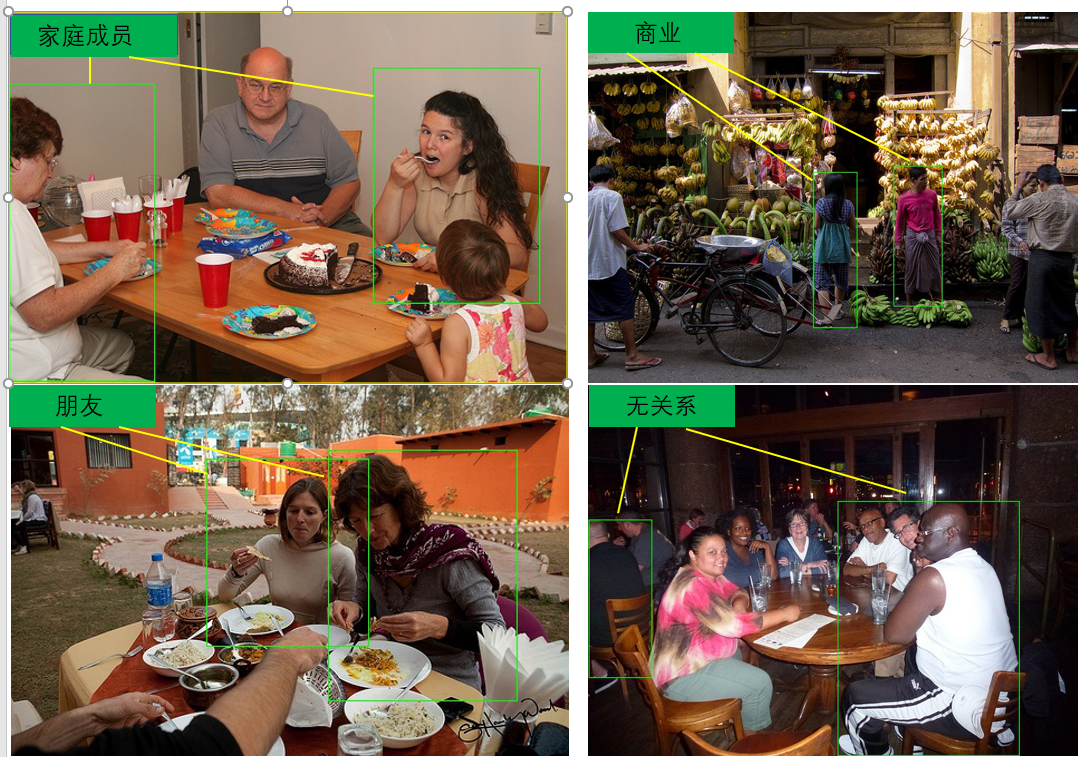
\includegraphics[width=0.95 \textwidth,clip]{example-1.png}
	%\hspace{0.02\textwidth}
	%\vspace*{-0.08cm}
    \caption{PISC数据集中的一些图片例子}
	\vspace*{-3.5mm}
	\label{fig:intro-example}
\end{figure}
\looseness=-1

既然社会关系理解对于理提升上述任务的关键资源,那么自然而然的,如何准确的理解社会关系成为需要研究者需要攻克的课题。一方面,一张图片的社会关系可以通过众包的方式,人工标注得到,比如现有的数据集PISC\cite{li2017dual-glance}和PISC-relation\cite{sun2017a}。当然,自动端到端的方法包括基于人脸特征、年龄、人的头部特征等特征信息的\cite{sun2017a,zhang2015learning}。还有利用周边环境的信息的模型\cite{li2017dual-glance,wang2018deep},这些模型通常需要一个物体检测器或者检测器中RPN(region proposal network),这都是需要引入额外的标注框或者预训练模型。也有通过对周边物体和社会关系共现的统计,例如``computer''和``professional''共同出现的概率较大,如果识别出存在``computer'',那么当前的关系很大概率是``professional'',通过神经网络引入这些先验知识来提升预测的准确率。这些自动识别社会关系的模型虽然不断在进步,但是从实验结果来看,他们与人工标注的准确率还是存在很大鸿沟,离实际的应用还存在很大的距离。

然后,现有的学习模型大都倾向于利用外部的知识来辅助理解图片的社会关系场景,但是得到这些外部知识需要额外的人工标注,这是一件耗时耗力的工作,或者一些统计得到的先验知识同样包含一些噪音,这也直接引出了到底是否应该引入外部知识,例如是否利用周边物体的信息,以及如何在缺乏这些信息的情况下取得好的实验效果。受到场景图谱生成的启发,场景图谱的概念最初是在2015年由Johnson 等人\cite{johnson2015image}提出的,是用于描述图片的一种新的半结构化的方式,基本组成单位是视觉三元组,形式为(头实体,关系,尾实体)。受到该领域下xu(2017)\cite{xu2017scene}的工作首先将整张图片输入,考虑到图片中不同视觉三元组之间的相互影响。例如,当知道``马在草地上''倾向于提高检测到``人骑着马''这条视觉三元组。对于社会关系检测的场景,如果图片中包含三个人对,其中两个人对的社会关系是``朋友'',那么第三条关系的的社会关系会倾向也是``朋友''或者其他的亲密关系,而不是``无关系''。直观上来说,这个是成立的,因此我们可以利用这当前场景下的其他的关系的来推理出当前的关系。

本论文主要研究如何将前文提到的关系场景的上下文信息引入社会关系理解的框架中。本文的出发点完全区别于Li(2017)\cite{li2017dual-glance}和Wang(2018)\cite{wang2018deep}的工作,
,对于关系特征的提取方法采用和Li\cite{li2017dual-glance}相同的策略。论文的切入点如图例\ref{fig:intro-example-2},图上六个人对的关系有五对是``朋友''关系,其中只有一对``奶奶-孙女''的关系,因此当前的图片应该是一个朋友聚会的场景拍下的。如果我们想推理出其中一个人对的关系并且已经知道其他部分人对的关系,那么直观的,我们会通过对已经知道的关系进行一个场景的判断,从而推理当前人对的关系到底是什么。在当前例子中,如果已经知道了2对或者3对都是``朋友''关系,那么当前的人对大概率也是``朋友''关系。因此,类似于前文提到的场景图谱的生成,以及现有的社会关系理解的研究现状,将当前的工作成为社会关系图谱生成
(social graph generation)。
\begin{figure}[htpb]
	\centering
	%	\includegraphics[width=0.48 \textwidth, trim=10 10 10 80,clip]{./pic/example_new.pdf}
	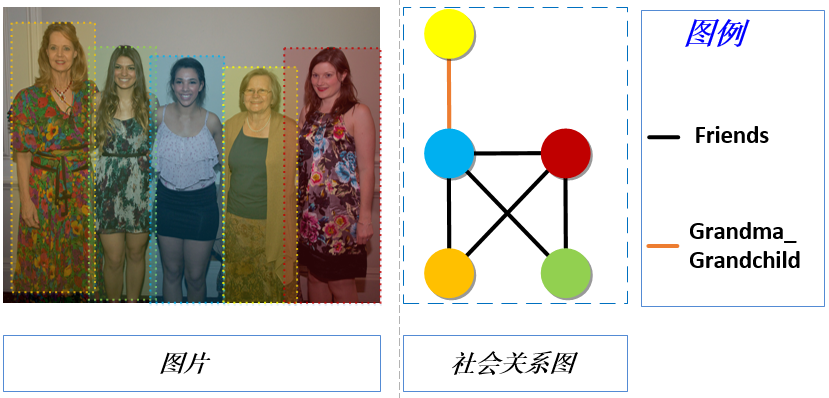
\includegraphics[width=0.95 \textwidth,clip]{example-2.png}
	%\hspace{0.02\textwidth}
	%\vspace*{-0.08cm}
    \caption{本论文动机的示例图,该图片来自PIPA-relation数据集,其中图片中对应阴影颜色的人对应社会关系图的部分,图上节点间的边表示他们之间的社会关系}
	\vspace*{-3.5mm}
	\label{fig:intro-example-2}
\end{figure}
\looseness=-1

在上述的介绍中,我们分别提到了两方面的相关内容,一方面社会关系理解的意义和作用,另外提到了与社会关系同属视觉理解领域的场景图谱的生成,收到这些工作的影响,可以列出他们的共性和特性如下:
\begin{enumerate}
    \item 场景图谱的基本组成是视觉三元组,社会关系图中是人对和人对间的社会关系,但是场景图谱中并没有人的的类别的概念,社会关系图中节点间的社会关系与人的类别无关。
    \item 场景图谱中的关系类别较多,有80-100个类别,但是在社会关系中,现有数据集不同粒度的关系类别分别为3、6、16,数量上远远不一样。并且在场景图谱中,关系的类型主要以空间关系为主,少量含有语义的关系,但是在社会关系图中,除了``无关系''和空间存在较大关联,其他的均为语义的关系。
    \item 与现有研究工作的区别是,之前的方法均将同一张图片上的不同人之间的关系割裂来看,但是他们间的关系互相影响,现有的研究工作忽略了这一点。
\end{enumerate}

要想解决社会关系理解问题,一种可行的方法是借助场景中除了人以外其他的信息,由于现有的数据集并没有标注其中的物体信息,所以需要借助额外的检测模型,但是由于模型的准确率的原因,会引入相当一部分的噪音,我们不能简单的加入这些信息,或者说我们是否需要加入这部分信息。其次是借助场景图谱生成的思想,认为一张图片中所有人对的社会关系不是割裂开的,是一同生成的,并且它们之间是相互影响的,但是由于场景图谱和社会关系图的区别,我们需要设计一个在社会关系理解人物下人对关系之间的交互机制。

\section{研究现状}

\subsection{视觉关系理解的应用}
在计算机视觉领域,社会关系信息被探索来提升几个常见的任务,例如人的轨迹预测\cite{kim2015brvo,robicquet2016learning}、 多目标追踪\cite{chen2012discovering,qin2012improving}和群体活动识别
\cite{direkoglu2012team,lan2012social,lan2012discriminative}。例如,在Deng等人(\cite{deng2016structure})群体活动识别的任务中,群体活动识别需要推理出图上人之间的结构信息,当前的方法是判断每个个体的动作,并且判断图上人之间的关系。但是由于图片特征的复杂和不确定性,这两个任务都是很有挑战的,推断出图上的结构信息能帮助排除一些未参与群体活动的人,得到更好的预测结果。因此预测这些人之间的社会关系能有助于群体活动识别。如图例\ref{fig:deng-example}所示,利用深度学习模型得到的人的表征和场景的表征后,如果知道了图例中第三个人和另外两个人之间不存在关系的情况下,排除第三个人对任务判断的影响。能更为容易的得出当前的群体活动场景是``waiting''。如Alahi(2016)\cite{alahi2016social}、robicquet等人(2016)\cite{robicquet2016learning}隐含的引入了社会性的约束来预测符合社会常识规则的人类运动轨迹,利用LSTM网络在序列任务的优越性,同时设计了特殊的池化模块来考虑邻居的运动走向。但是可以通过加入已经识别好的社会关系,即人与人之间的相互作用,当作常识规则来增强对运动轨迹预测鲁棒性和准确率。
\begin{figure}[htpb]
	\centering
	%	\includegraphics[width=0.48 \textwidth, trim=10 10 10 80,clip]{./pic/example_new.pdf}
	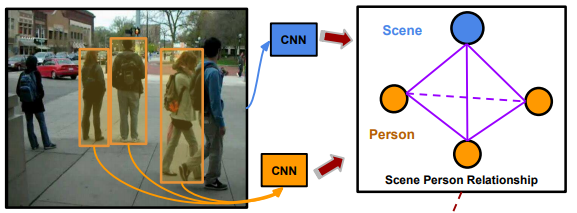
\includegraphics[width=0.95 \textwidth,clip]{deng-example.png}
	%\hspace{0.02\textwidth}
	%\vspace*{-0.08cm}
    \caption{来自Deng等人\cite{deng2016structure}的示例图}
	\vspace*{-3.5mm}
	\label{fig:deng-example}
\end{figure}
\looseness=-1

在社会关系理解之外,也有很多的工作明确的关注社会属性和社会结构的识别Wang等人(2010)\cite{wang2010seeing}通过分析个人的相册集来实现个人的家庭社会关系识别,
亲属关系验证\cite{dibeklioglu2013like,fang2010towards,xia2012understanding}和亲属识别\cite{chen2012discovering,guo2014graph}等任务也被广泛的探索和研究。Zhang等人(2015)\cite{zhang2015learning}研究人的面部表情,例如友好的、统治的,这些信息有助于推断社会关系。而在基于视频分析的领域中,Ding等人\cite{ding2014learning}从电影中挖掘演员的关系。社会关系理解在某个方面和社会信号处理\cite{vinciarelli2009social},社会信号处理的目标是利用多个传感器理解社会信号和社会行为,例如角色识别、影响力排名和统治力检测等\cite{hung2007using,rienks2006detection,salamin2009automatic}。但是本文关注的社会关系理解本质上不同于前面提到的这些工作,和基于面部表情的社会关系检测不同的是,本文的研究图片中的个体往往是姿态和朝向都不确定的。此外,本文着重的社会关系是更普遍的社会关系,而不是家庭相册中的亲属关系。与视频任务不同的是,本文关注的一张图片中的视觉信息。

前面的社会关系理解的工作大多数都是利用向量化的社会关系来帮助推理,与社会关系理解同属同一个视觉关系理解任务类别,即场景图谱的生成,又或者称为视觉关系检测。该任务的最早是Johnson等人于2015年提出的
\cite{johnson2015image},是一种用于描述图片场景的新的方式,与本文工作不同的是,场景图谱中的主要组成部分不仅包括人,还包括很多日常物体,如图\ref{sg-example}所示。两个工作最核心的挑战在于推理出物体之间的关系。由于场景图谱常用于图片检索\cite{johnson2015image},Marino(2017)\cite{marino2017the}利用得到场景图谱结合图神经网络提高图片的分类效果。在以上关于视觉信息理解的两个方向上,都有大量的工作提出,分别用于解决不同场景的问题,因此如何更好的实现视觉理解这个难题自然而然的成为许多研究者想要攻克的难题。对于场景图谱来说,本文的工作主要受到了以下几个工作的启发。Xu等人(2017)对于场景图谱进行建模,分别包含物体节点和关系节点,然后采用Message Passing的方式进行迭代。通过相邻的节点或边对目标节点或边进行约束,从而对这些特征进行微调,达到提升的效果。Yang等人(2018)利用图卷积网络进行不同节点之间的Message passing来达到约束的效果。融合自然语言知识提出的VRD模型\cite{liang2018visual},本文初始步骤中的特征提取工作中包含空间信息的提取便收到该工作的启发。
\begin{figure}[htpb]
	\centering
	%	\includegraphics[width=0.48 \textwidth, trim=10 10 10 80,clip]{./pic/example_new.pdf}
	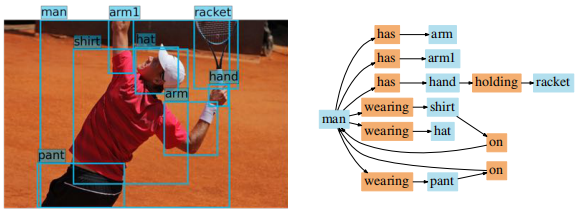
\includegraphics[width=0.95 \textwidth,clip]{sg.png}
	%\hspace{0.02\textwidth}
	%\vspace*{-0.08cm}
    \caption{场景图谱\cite{xu2017scene}的示例图}
	\vspace*{-3.5mm}
	\label{fig:sg-example}
\end{figure}
\looseness=-1

\subsection{社会关系理解的方法}
而对于社会关系理解,作为最早的工作,wang等人(2010)开始引入家庭关系当前背景来识别人之间亲属关系。在后来的工作中\cite{dibeklioglu2013like,xia2012understanding,chen2012discovering},为了捕获这些社会关系展现出来的一些规律,探索了面部表情和属性等用于亲属关系识别和验证。并且为了促进社会关系理解领域的研究和发展,Li\cite{li2017dual-glance}和Sun\cite{sun2017a}构建了大规模的数据集,并且利用深度学习的模型直接从图片中学习来识别关系。对于Sun构建的数据集PIPA-Relation,该数据集的关系包括5个领域,然后基于这5个领域又划分为16条关系。同样,Li基于关系模型理论,定义了一系列的关系列别,包含两个不同层次关系的划分,粗粒度的3类关系和细粒度的6类关系。在Sun(2017)等人的工作中,不仅提出了两个关系粒度的数据集,而且提出了Dual-glance模型。该模型是一个流水线的模型,并且包括两个模块,主要的的创新点在于利用人对周边的物体信息来提升关系检测的效果。Wang(2018)等人提出了基于知识图谱的深度推理模型,通过图门控神经网络引入物体的社会关系的共现的常识知识来实现物体和关系之间的推理,本质上还是利用周边的物体信息,但是在Dual-glance中,用到只是周边的物体区域,并不需要准确的识别出物体区域的物体类别。

在关系理解领域,除了社会关系理解,还有视觉关系检测任务。与社会关系检测不同,视觉关系检测首先依赖于一个物体检测器识别出所有的物体,然后依次两两识别两个物体存在的关系。在社会关系检测中,物体的类别只有人,并且一张图片中的人往往不会太多。Lu等人\cite{lu2016visual} 提出首先提出VRD 模型,利用自然语言得到的词向量作为先验知识来帮助单条三元组的检测。后来,Zhang 等人\cite{zhang2017visual} 提出VTranE 模型,模拟知识图谱中关系翻译,即$h + r = t$,本质上还是一个关系的分类器。但是并没有考虑到视觉关系的复杂度,并且不同于自然语言的状态翻译。Li (2017)等人\cite{li2017scene}进一步提出了多任务混合模型,任务包括场景图谱、区域描述生成、物体识别。和VRD类似,通过多种任务联合训练,引入额外的信息。Zellers 等人(2018)\cite{zellers2018neural}提出motif-net,通过分析数据集得出关视觉关系严重依赖头尾实体的类别,利用双向循环神经网络对物体类别编码信息进行编码处理,提升了物体识别的准确度,进而提升了任务的效果。

\subsection{研究现状小结}
当前社会关系理解领域的工作主要方式是引入额外的信息,例如引入面部表情和属性、年龄等。以及通过物体检测的方法识别出当前场景中的物体,来优化单纯通过提取人的区域的表征。最新的工作尝试引常识知识,对物体和关系间的常识知识进行表征来提高模型的效果。无论是采用额外的物体检测模型还是通过引入常识知识,都是外部信息,不可避免的需要额外的消耗或引入一些噪声。同时,对于人的轨迹预测、 多目标追踪 和群体活动识别任务,引入社会关系的信息能有效的提高这些任务的效果。因此,如何利用更少的信息,来提升预测效果是当前的一大挑战。同时以消息传递机制为技术栈的微调机制的方法在场景图谱,同属视觉理解领域得到了运用,在一定程度上解决了场景图谱的生成问题。然而,由于场景图谱和社会关系任务理解两个不同人物上的区别,如何在社会关系理解中引入消息传递机制仍然面临很多的挑战

\section{本文工作}

本文首先通过介绍现有的社会关系理解最新研究工作,分析它们的模型设计的出发点,模型的结构,分析这些工作的忽略的信息,即没考虑到整张图片不同的人对的关系之间的互相影响。因此,本文提出了一个考虑到同一张图片不同关系之间存在交互的模型:包含人对消息传递机制的模型,人对关系网络(Person-pair Relation Network),简称PPRN,最后把该模型应用到社会关系理解的任务中,在两个公开数据集上做了对比实验。
本文提出的PPRN模型包括以下模块:
\begin{enumerate}
    \item 特征抽取模块,对于特征抽取模块,本文采用一个ResNet101\cite{he2016deep}抽取两个人的单独区域的特征,同时另外一个ResNet101抽取人对区域的特征。同时,对于这个模块,人对的位置信息也加入了最后的表征向量中。
    \item 消息传递模块,本文首次尝试在社会关系理解任务中引入多个人对之间的关系的想法。对于消息传递模块,利用以GRU单元为组件的RNN来实现消息传递,并且设置多个迭代步,实现消息传递和池化模块的交互。采用RNN 最后隐藏层的输出作为图片中人对的关系表征。
    \item 消息池化模块,本文设计了一个交互机制来处理人对之前的关系的信息,同时利用注意力机制来提高模型的表现效果。
    \item 融合周边物体信息模块,与Dual-galnce\cite{li2017dual-glance}类似,本文在经过消息传递、池化两个模块后得到的人对关系编码,利用注意力机制得到周边物体区域特征编码。两部分特征融合后,进行最后的关系分类。
\end{enumerate}
在实验中,本文在两个公开数据集上验证了\textbf{PPRN}模型的有效性,它们分别是PIPA-Relation和PISC,其中PISC包括两个粒度的子数据集PISC-coarse和PISC-fine。与此同时,在加入最后的周边物体信息模块后,模型效果轻微下降。
接着,本文进一步通过案例研究的方法分析了\textbf{PPRN} 模型的具体效果。从实验结果可以看出,\textbf{PPRN}模型在与其他基准模型的比较中取得了在两个数据集上取得了最优的结果,说明了引入不同关系之间交互的消息传递机制在社会关系理解为基础场景中的重要性。

\section{论文结构}

全文的组织结构描述如下:

第1章:介绍了社会关系理解的相关背景,点明了当前社会关系理解存在的缺点,由此引入了同属视觉关系理解人物的场景图谱,分析并总结了场景图谱的研究现状,并针对两者的共同点引出社会关系理解的提升方案。

第2章:首先介绍了图像领域的视觉信息抽取的方法,从简单的神经网络、卷积神经网络、以及残差网络等介绍。之后基于前面的神经网络的知识,介绍了现有工作中常用的物体检测与识别的方法,并进行了讨论与对比。然后详细介绍了当前社会关系理解模型的各个部件,最后对本章内容进行了总结。

第3章:针对社会关系理解的特点,提出了基于消息传递机制的社会关系理解方法,设计了图像中不同人对的社会关系交互的PPRN模型,并且具体介绍了模型的细节。同时实现了结合周边物体信息的模块,分析了模型的设计原则和具体细节。

第4章:首先介绍了两个在社会关系理解领域常用的数据集,并对PPRN模型在不同关系粒度的数据集上进行了训练和测试,接着针对实验结果进行了分析。然后还进一步通过案例研究的方式分析了PPRN在社会关系理解的变现。

第5章:总结了本文的研究工作,并且提出了进一步的研究展望。




\clearpage{\pagestyle{empty}\cleardoublepage}       %本有
% !Mode:: "TeX:UTF-8"

\chapter{����о�}

Ҳ����һ�ֽṹ������о����ڵ�һ�£��ӵڶ��¿�ʼ�����Լ����о���

\section{��һ��}

�Ǻ�

\subsection{��һ�ڵĵ�һС��}

����

\subsection{��һ�ڵĵڶ�С��}

�ٺ�

\section{�ڶ���}

aa

\subsection{�ڶ��ڵĵ�һС��}

bb

\section{��һ��}

�Ǻ�

\subsection{��һ�ڵĵ�һС��}

����

\subsection{��һ�ڵĵڶ�С��}

�ٺ�

\section{�ڶ���}

aa

\subsection{�ڶ��ڵĵ�һС��}

bb

\section{��һ��}

�Ǻ�

\subsection{��һ�ڵĵ�һС��}

����

\subsection{��һ�ڵĵڶ�С��}

�ٺ�

\section{�ڶ���}

aa

\subsection{�ڶ��ڵĵ�һС��}

bb


\clearpage{\pagestyle{empty}\cleardoublepage}       %本有
%\include{body/mns}
%\clearpage{\pagestyle{empty}\cleardoublepage}       %本有
%\include{body/momns}
%\clearpage{\pagestyle{empty}\cleardoublepage}       %本有
%\include{body/experiment}
%\clearpage{\pagestyle{empty}\cleardoublepage}       %本有
%% !Mode:: "TeX:UTF-8"

\chapter{总结与展望}
\label{ch:conclusion}

\section{本文总结}

近年来,随着深度学习方法在计算机视觉领域的广泛应用,基于图像理解的应用也逐渐增多,随之各种任务数据集的构造和应用的落地。但是基于图片的高层次推理和理解仍然是待解决的难题,例如图像的视觉理解,以及本文关注的社会关系理解人物。与此同时,随着人们的研究的深入进展,如何利用更少的信息和人工干预来提升社会关系理解任务的效果是一大挑战。此外,在视觉理解领域的另外一个方向,基于消息传递、图网络等技术生成的场景图谱在各大领域的成功应用,例如图像问答和图像检索。但是由于两者存在许多不同点,在社会关系理解领域引入场景图谱生成的方法是另外一大挑战。
本文的主要工作和贡献点总结如下:
\begin{enumerate}
    \item 针对提出的挑战,本文首先弄明白了现有关系理解方法的研究现状,分析了现有方法的研究现状,现有方法忽略了一张图片人对的关系之间互相影响的信息。即现有的方法需要额外的检测标注。其次,调研了现有场景图谱生成工作,明确了社会关系理解和场景图谱理解的各项概念。社会关系理解的目的是识别出给定一对人的的社会关系。
    \item 接下来,本文充分考虑了同一场景下多个人对的社会关系间互相这一因素,提出了人对关系网络(PPRN),这是首个在社会关系理解任务上引入人对关系的交互模型。针对性的设计了迭代的消息传递和池化模块来融合交互信息。主要包括3个模块:视觉特征提取模块、消息传递和消息池化模块。视觉特征提取模块主要是由2部分组成,个体CNN和联合CNN,采用的是预训练的ResNet-101,结合位置信息后得到关于人对关系的特征编码向量。传递和消息池化主要是利用迭代的门控循环神经网络实现推理,并且在每个神经元之前都采用消息池化的机制融合其他人对的信息。此外,本文还实现了融合周边物体信息模块,得到物体特征的特征编码向量,进一步验证模型的效果。
    \item 为了验证本文所提出的PPRN模型的有效性,本文在两个大规模的数据集上进行了相关的实验、主要的评价指标包括每个关系类别热召回率以及mAP。采用每个关系类别的召回率是因为每个关系类别的训练样本存在数据不均衡的情况,与此同时还需要在训练集进行过采样和降采样。mAP综合考虑召回率和准确率的效果。实验结果说明PPRN模型在社会关系理解任务上展现了优秀的性能,说明了考虑人对关系上下文的重要性。同时,基于低层次特征抽取模型得到的编码,再进行高层次的推理,是本文的核心点。
\end{enumerate}

\section{研究展望}

基于对社会关系理解的分析以及本文提出对各项相关任务的分析、相关技术的考量,基于本文的基础,未来的研究可以是以下方面开展:
\begin{enumerate}
    \item 将现有的视觉关系检测的工作引入到社会关系检测中,人们对场景图谱的研究相当深入,视觉三元组在图像问答和图片检索上发挥了很大的作用。同时,现有的社会关系理解的``人''并没有id或者名称,可以结合人脸识别的方法进一步给识别出人的id,建立一个整体的图像社会关系图谱。
    \item 现有模型挖掘的特征包括周边的物体上下文、关系上下为难均为场景这一粒度的,可以尝试加入更细粒度的。例如人的性别特征,这样的特征在区分{\it Friends}和{\it Couple}等容易混淆的气密关系的时候时能起到关键的作用,例如相同性别一般不可能是{\it Couple},而是其他的亲密关系。
    \item 可以将视觉领域的社会关系理解拓展到视频领域的,
\end{enumerate}


%\clearpage{\pagestyle{empty}\cleardoublepage}       %本有

%%%%%%%%%%  参考文献  %%%%%%%%%%
\titleformat{\chapter}{\centering\sihao\hei}{\chaptername}{2em}{}
\defaultfont
%\bibliographystyle{TJUThesis}
\bibliographystyle{references/TJUThesis}        % bst文件名,注意不要后缀
\phantomsection
\markboth{参考文献}{参考文献}
\addcontentsline{toc}{chapter}{参考文献}        % 参考文献加入到中文目录
%\nocite{*}                                     % 若将此命令屏蔽掉,则未引用的文献不会出现在文后的参考文献中
\bibliography{references/reference}             % bib文件名
\include{references/reference}
\clearpage{\pagestyle{empty}\cleardoublepage}   %本有
\include{appendix/cmpresult-A}               %附录 实验结果表
\clearpage{\pagestyle{empty}\cleardoublepage}
\include{appendix/cmpresult-B}               %附录 实验结果表
\clearpage{\pagestyle{empty}\cleardoublepage}
%% !Mode:: "TeX:UTF-8"

\markboth{攻读硕士学位期间发表学术论文情况}{攻读硕士学位期间发表学术论文情况}
\addcontentsline{toc}{chapter}{攻读硕士学位期间发表学术论文情况}
%\setcounter{page}{1}       % 如果需要从该页开始从 1 开始编页,则取消该注释
\chapter*{攻读硕士学位期间发表学术论文情况}

\begin{enumerate}
	% 盲审时
	\item Understanding Social Relationship with Person-pair Relations. 投稿于IJCAI-2019(ccf推荐A类会议),学生第一作者,审稿中
    \item 一种基于二次主题空间投影的场景图谱低维空间嵌入方法; (学生第一作者,申请未公开)
	% 提交时
	%\item Authors. The paper title [J/C...]. Publish whereabout, 2014, 21(3): 288-291. (提交时)
\end{enumerate}

% 仍然有页码
%\thispagestyle{empty}
                       % 攻读硕士学位期间发表学术论文情况
\clearpage{\pagestyle{empty}\cleardoublepage}   %本有
% !Mode:: "TeX:UTF-8"

\markboth{致\quad 谢}{致\quad 谢}
\addcontentsline{toc}{chapter}{致\quad 谢} % 添加到目录中
\chapter*{致\quad 谢}

谨此向我的导师张三教授致以衷心的感谢和崇高的敬意!本论文的工作是在张老师的悉心指导下完成的。在传授予我专业知识和宝贵经验的同时,张老师以其严谨的治学态度和精益求精的工作作风不断促进论文相关工作的进行,使我受益匪浅。
 
在攻读硕士的这三年里,导师和实验室的同学们不仅为我创造了优越的科研和学习环境,使我得以在计算机科学领域中自由翱翔,同时在思想上、人生态度和意志品质方面给予了谆谆教诲,这些教益必将激励着我在今后的人生道路上奋勇向前。特别感谢实验室的甲师兄、乙同学以及其他师弟师妹,他们不仅在学术上给了我许多指引和建议,而且在生活上予以帮助,从他们身上我学到了很多知识。

感谢王五老师及其实验室的同学在领域一、领域二方面的学习给予我的帮助。他们开创性的研究拓展了我的学术视野,无数次的争论和探讨使我的研究工作有了长足的进展。

由衷感谢我的室友A、B和C同学,以及其他经常到我们宿舍进行学习交流的D、E、F和G同学,是他们令我的学习生活都更加充满动力。
衷心的感谢我的父母和其他亲朋好友对我的关心、支持和理解,没有他们对我的关心、鼓励和支持,我无法完成现在的硕士学业。 

最后,感谢所有曾经教育和帮助过我的所有老师。衷心地感谢为评阅本论文而付出宝贵时间和辛勤劳动的专家和教授们!

% 如果需要加名字和日期(日期根据生成文档日期变更)
\begin{flushright}
  \begin{tabular}{cl}
    李四 & \\
    二零一四年\CJKnumber{\the\month}月\CJKnumber{\the\day}日 & 
  \end{tabular}
\end{flushright}

             % 致谢
%\clearpage{\pagestyle{empty}\cleardoublepage}
\clearpage
\end{CJK*}                                      % 结束中文字体使用
\end{document}                                  % 结束全文
